% ------------------------------------------------------------------------------
% TYPO3 Version 9.3 - What's New - Chapter "Changes for Integrators" (English Version)
%
% @author	Michael Schams <schams.net>
% @license	Creative Commons BY-NC-SA 3.0
% @link		http://typo3.org/download/release-notes/whats-new/
% @language	English
% ------------------------------------------------------------------------------
% LTXE-CHAPTER-UID:		3a9852ea-e2360d9d-1ff5eec1-a7de3f9f
% LTXE-CHAPTER-NAME:	Changes for Integrators
% ------------------------------------------------------------------------------

\section{Changes for Integrators}
\begin{frame}[fragile]
	\frametitle{Changes for Integrators}

	\begin{center}\huge{Chapter 2:}\end{center}
	\begin{center}\huge{\color{typo3darkgrey}\textbf{Changes for Integrators}}\end{center}

\end{frame}

% ------------------------------------------------------------------------------
% LTXE-SLIDE-START
% LTXE-SLIDE-UID:		0e80eecb-f66842d4-e73c50c8-c2bb58a6
% LTXE-SLIDE-TITLE:		...
% LTXE-SLIDE-REFERENCE:	#84843 - Use no-cookie domain for youtube by default
% ------------------------------------------------------------------------------

\begin{frame}[fragile]
	\frametitle{Changes for Integrators}
	\framesubtitle{No-cookie Domain for YouTube Videos}

	% decrease font size for code listing
	\lstset{basicstyle=\smaller\ttfamily}

	\begin{itemize}
		\item YouTube videos are rendered by accessing the no-cookie domain
			\url{https://www.youtube-nocookie.com} by default
		\item The regular domain \texttt{www.youtube.com} can be forced by
			the following TypoScript configuration, if required:

			\begin{lstlisting}
				lib.contentElement {
				  settings {
				    media {
				      additionalConfig {
				        no-cookie = 0
				      }
				    }
				  }
				}
			\end{lstlisting}

	\end{itemize}

\end{frame}

% ------------------------------------------------------------------------------
% LTXE-SLIDE-START
% LTXE-SLIDE-UID:		0e80eecb-f66842d4-e73c50c8-c2bb58a6
% LTXE-SLIDE-TITLE:		General Data Protection Regulation
% LTXE-SLIDE-REFERENCE:	#84843 - Use no-cookie domain for youtube by default
% LTXE-SLIDE-REFERENCE:	GDPR Initiative: https://forge.typo3.org/issues/84776
% ------------------------------------------------------------------------------

\begin{frame}[fragile]
	\frametitle{Changes for Integrators}
	\framesubtitle{General Data Protection Regulation}

	\begin{itemize}
		\item Scheduler task can be activated to anonymize IP addresses in
			several database tables after a certain period of time.\newline

			For example table \texttt{sys\_log}, after 30 days:
			\begin{figure}
				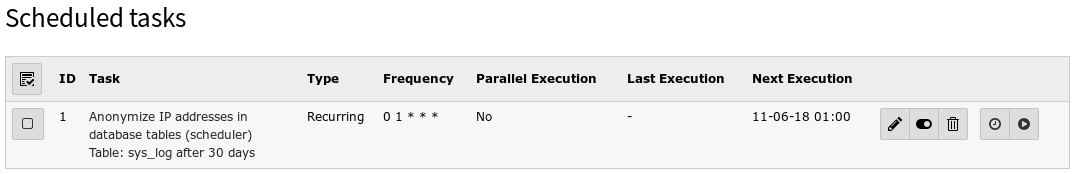
\includegraphics[width=1\linewidth]{ChangesForIntegrators/IpAnonymizationSchedulerTask.png}
			\end{figure}

		\item The \href{https://typo3.com/blog/tag/gdpr/}{TYPO3 GmbH Blog}
			contains further information about GDPR
	\end{itemize}

\end{frame}

% ------------------------------------------------------------------------------
% LTXE-SLIDE-START
% LTXE-SLIDE-UID:		0e80eecb-f66842d4-e73c50c8-c2bb58a6
% LTXE-SLIDE-TITLE:		FE/BE User Accounts and Passwords
% LTXE-SLIDE-REFERENCE:	#85026 - salted passwords changes
% ------------------------------------------------------------------------------

\begin{frame}[fragile]
	\frametitle{Changes for Integrators}
	\framesubtitle{FE/BE User Accounts and Passwords}

	% decrease font size for code listing
	\lstset{basicstyle=\tiny\ttfamily}

	\begin{itemize}
		\item Plain text passwords are not longer possible for BE/FE users at all
		\item Inactive FE/BE user records can now be removed from the database by
			adding scheduler task "Table garbage collection task" and enabling
			"Clean all available tables"\newline
			\smaller
				(data that does not exist, cannot be compromised in case of a
				security breach)
			\normalsize

			\begin{lstlisting}
				<?php
				$tableGarbageCollectionTask = \TYPO3\CMS\Scheduler\Task\TableGarbageCollectionTask::class;
				$GLOBALS['TYPO3_CONF_VARS']['SC_OPTIONS']['scheduler']['tasks'][$tableGarbageCollectionTask]
				  ['options']['tables'] = [
				  'be_users' => [
				    'dateField' => 'lastlogin',
				    'expirePeriod' => 30
				  ]
				];
			\end{lstlisting}

		\item See \href{https://docs.typo3.org/typo3cms/extensions/scheduler/Installation/BaseTasks/Index.html}{documentation}
			for further details
	\end{itemize}

\end{frame}

% ------------------------------------------------------------------------------
% LTXE-SLIDE-START
% LTXE-SLIDE-UID:		f38ee3cb-51d1aa0a-4f6884bf-adadc9e3
% LTXE-SLIDE-TITLE:		"Duplicate" Button
% LTXE-SLIDE-REFERENCE:	#84749 - Hide "duplicate" button by default
% ------------------------------------------------------------------------------

\begin{frame}[fragile]
	\frametitle{Changes for Integrators}
	\framesubtitle{"Duplicate" Button}

	% decrease font size for code listing
	\lstset{basicstyle=\smaller\ttfamily}

	\begin{itemize}
		\item Button to duplicate a content element is now hidden by default
		\item Visibility can be configured by user TSconfig ("1" = enabled):

			\begin{lstlisting}
				options.showDuplicate = 1
				options.showDuplicate.[table] = 1
			\end{lstlisting}

	\end{itemize}
	\vspace{-0.5cm}
	\begin{figure}
		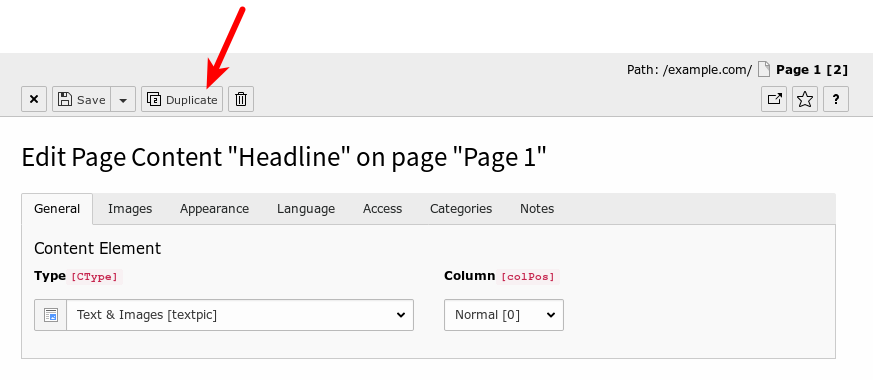
\includegraphics[width=0.8\linewidth]{ChangesForIntegrators/DuplicateButtonHiddenByDefault.png}
	\end{figure}

\end{frame}

% ------------------------------------------------------------------------------
% LTXE-SLIDE-START
% LTXE-SLIDE-UID:		0e80eecb-f66842d4-e73c50c8-c2bb58a6
% LTXE-SLIDE-TITLE:		HTML5 Date Form Element
% LTXE-SLIDE-REFERENCE:	#82511 - EXT:form add HTML5 date form element
% ------------------------------------------------------------------------------

\begin{frame}[fragile]
	\frametitle{Changes for Integrators}
	\framesubtitle{\texttt{EXT:form} HTML5 Date Form Element}

	% decrease font size for code listing
	\lstset{basicstyle=\tiny\ttfamily}

	\begin{itemize}
		\item The form framework contains a new form element "\texttt{Date}",
			including appropriate validator
		\item This is technically an HTML5 \texttt{'type=date'} attribute
			(see \href{https://www.w3.org/TR/2011/WD-html-markup-20110405/input.date.html}{w3c.org})
		\item Example (including the "DateRange" validator):

			\begin{lstlisting}
				type: Date
				identifier: date-1
				label: Date
				defaultValue: '2018-03-02'
				properties:
				  displayFormat: 'd.m.Y'
				  fluidAdditionalAttributes:
				    min: '2018-03-01'
				    max: '2018-03-30'
				    step: '1'
				validators:
				  -
				    identifier: DateRange
				    options:
				      minimum: '2018-03-01'
				      maximum: '2018-03-30'
			\end{lstlisting}

	\end{itemize}

\end{frame}

% ------------------------------------------------------------------------------
% LTXE-SLIDE-START
% LTXE-SLIDE-UID:		0e80eecb-f66842d4-e73c50c8-c2bb58a6
% LTXE-SLIDE-TITLE:		Destructive Database Schema Changes
% LTXE-SLIDE-REFERENCE:	#85160 - Non destructive database schema changes in extension manager
% ------------------------------------------------------------------------------

\begin{frame}[fragile]
	\frametitle{Changes for Integrators}
	\framesubtitle{Destructive Database Schema Changes}

	\begin{itemize}
		\item If an extension is installed or updated via the Extension Manager,
			and \textit{destructive} database changes are required, these changes
			are not applied automatically anymore
		\item "Destructive" changes are for example changes of existing columns,
			removal of a column, index or table definition, etc.
		\item To review and possibly execute these outstanding database updates,
			go to: ADMIN TOOLS → Maintenance → Analyze Database Structure\newline
	\end{itemize}

	\vspace{-0.4cm}

	% Translators: remove the illustration below, if it does not fit on the
	% slide, e.g. in case your language requires more space. The illustration is
	% not really required, just "nice to have".

	\begin{figure}
		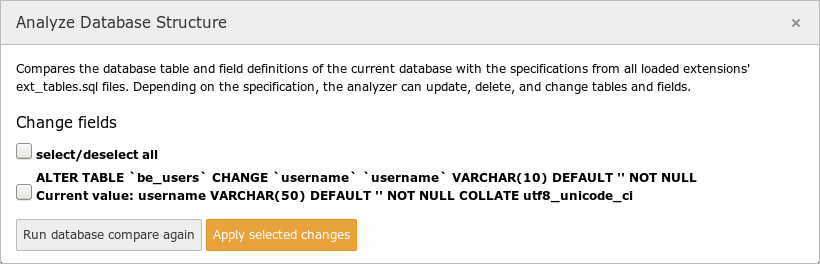
\includegraphics[width=0.6\linewidth]{ChangesForIntegrators/DestructiveDatabaseChanges.png}
	\end{figure}

\end{frame}

% ------------------------------------------------------------------------------
% LTXE-SLIDE-START
% LTXE-SLIDE-UID:		0e80eecb-f66842d4-e73c50c8-c2bb58a6
% LTXE-SLIDE-TITLE:		TypoScript Conditions
% LTXE-SLIDE-REFERENCE:	#84760 - TypoScript conditions for site and siteLanguage
% ------------------------------------------------------------------------------

\begin{frame}[fragile]
	\frametitle{Changes for Integrators}
	\framesubtitle{TypoScript Conditions}

	New TypoScript conditions:

	\begin{itemize}
		\item Condition for the properties of a site object

			\begin{lstlisting}
				[site = identifier = someIdentifier, base = https://example.com/]
				  page.30.value = foo
				[global]
			\end{lstlisting}

		\item Condition for the site language

			\begin{lstlisting}
				[siteLanguage = locale = de_CH.UTF-8, title = Switzerland]
				  page.40.value = bar
				[global]
			\end{lstlisting}

	\end{itemize}

\end{frame}

% ------------------------------------------------------------------------------
% LTXE-SLIDE-START
% LTXE-SLIDE-UID:		0e80eecb-f66842d4-e73c50c8-c2bb58a6
% LTXE-SLIDE-TITLE:		HMENU cObj and language IDs
% LTXE-SLIDE-REFERENCE:	#84775 - Extend HMENU to support auto filling of special.value for special=language
% ------------------------------------------------------------------------------

\begin{frame}[fragile]
	\frametitle{Changes for Integrators}
	\framesubtitle{\texttt{HMENU} cObj and language IDs}

	% decrease font size for code listing
	%\lstset{basicstyle=\tiny\ttfamily}

	\begin{itemize}
		\item \texttt{HMENU} content object now supports the auto filling of
			language IDs for language menus

			\begin{lstlisting}
				10 = HMENU
				10 {
				  special = language
				  special.value = auto
				}
  			\end{lstlisting}

		\item \texttt{special.value} list of comma separated language IDs
			(e.g. 0,1,2) or \texttt{auto} to load the list from site languages

	\end{itemize}

\end{frame}

% ------------------------------------------------------------------------------
% LTXE-SLIDE-START
% LTXE-SLIDE-UID:		0e80eecb-f66842d4-e73c50c8-c2bb58a6
% LTXE-SLIDE-TITLE:		View User TSConfig Data
% LTXE-SLIDE-REFERENCE:	#85017 - User TSConfig shown in Configuration module
% ------------------------------------------------------------------------------

\begin{frame}[fragile]
	\frametitle{Changes for Integrators}
	\framesubtitle{View User TSconfig Data}

	User TSConfig data of the currently logged-in user can be accessed at
	\textbf{System -> Configuration}

	\begin{figure}
		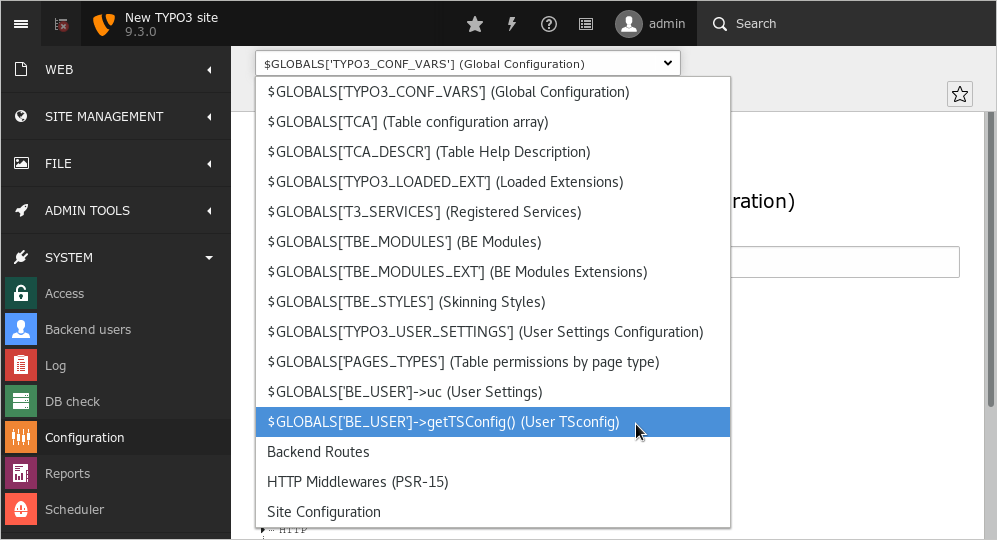
\includegraphics[width=0.75\linewidth]{ChangesForIntegrators/SystemConfigurationUserTSConfig.png}
	\end{figure}

\end{frame}

% ------------------------------------------------------------------------------
% LTXE-SLIDE-START
% LTXE-SLIDE-UID:		0e80eecb-f66842d4-e73c50c8-c2bb58a6
% LTXE-SLIDE-TITLE:		Miscellaneous
% LTXE-SLIDE-REFERENCE:	#69274 - Preserve image rotation if orient is saved in exif
% LTXE-SLIDE-REFERENCE:	#85147 - Render SEO meta tags in frontend
% LTXE-SLIDE-REFERENCE:	#84715 - Set exclude property for tt_content fields
% ------------------------------------------------------------------------------

\begin{frame}[fragile]
	\frametitle{Changes for Integrators}
	\framesubtitle{Miscellaneous}

	\begin{itemize}
		\item TYPO3 takes the image orientation stored as EXIF data into account,
			when reading dimensions and processing the image (e.g. scaling/cropping)
		\item SEO-related meta tags set in the page properties are now rendered
			in frontend by default
		\item The \textit{exclude} property is set for the following fields:

			\begin{itemize}
				\smaller
				\item \texttt{tt\_content.file\_collections}
				\item \texttt{tt\_content.filelink\_size}
				\item \texttt{tt\_content.filelink\_sorting}
				\item \texttt{tt\_content.filelink\_sorting\_direction}
			\end{itemize}

			\small
				Access permissions must be adjusted, if editors should be able
				to edit these fields!
			\normalsize

	\end{itemize}

\end{frame}

% ------------------------------------------------------------------------------
